\chapter{First Species of Counterpoint}

\begin{quotation}
    "With God's help, then let us begin composition for two voices. We take as a basis for this given melody or \cfcomma which we invent ourselves or select from a book of chorales. To each of these notes, now, should be set a suitable consonance in a voice above [\dots]."
    \textcite[p.27]{GaPEng}
\end{quotation}

The first species of counterpoint consists of one note by measure, note against note. In other words, only whole notes.
\begin{figure}[h]
    \centering
    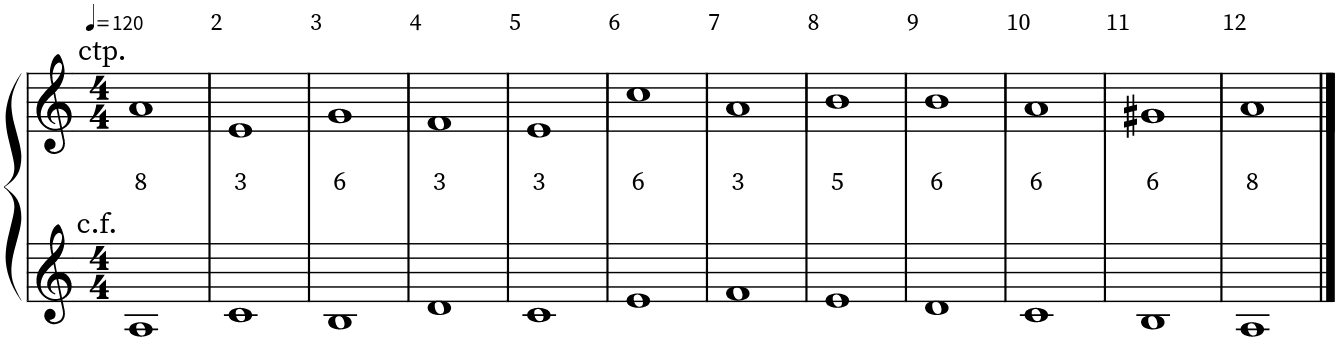
\includegraphics[height=\fhl]{Images/the_first_species.png}
    \caption{Example of a \species{1} ctp. \listen{Listen1SP} \listenyt{https://youtu.be/9yB4OGr4Cgk?t=14}}
\end{figure}

As a reminder, \textit{unless mentioned}, harmonic and melodic intervals are considered in absolute values. Moreover, harmonic intervals are modulo 12, so an octave interval is equivalent to a unison interval (see section \ref{sec:variables}).

\section{Formalization in English} \label{subsec:1SPEnglish}

\subsection{Harmonic Rules of the First Species}
\begin{enumerate}[wide, label=\bfseries 1.H\arabic*]
    \item\label{rule:allcons} \textit{All harmonic intervals must be consonances\footnote{This excludes dissonances which are seconds, fourths, and sevenths.}.} \textcite[p.53]{GaPFr}

    \begin{quotation}
        "[The master addressing his pupil] I shall explain to you. It is the simplest composition of two voices [\dots] which, having notes of equal length, consists only of consonances."
        \textcite[p.27]{GaPEng}
    \end{quotation}

    \item\label{rule:firstpcons} \textit{The first harmonic interval must be a perfect consonance\footnote{Perfect consonances are fifths and octaves (or unisons).}.} \parencite[p.54]{GaPFr}

    Perfect consonances are not those that bring the most harmony but those that give the most sense of stability and rest. They clarify the key and provide a strong foundation for the entire musical work. This rule applies to all species.

    \item\label{rule:lastpcons} \textit{The last harmonic interval must be a perfect consonance.} \parencite[p.54]{GaPFr}

    Same logic as the previous rule. This one also applies to all species.

    \item\label{rule:keytone} \textit{The key tone is tuned according to the first note of the \cfdot} \parencite[p.56]{GaPFr}

    As seen in section \ref{sec:generalenglish}, Fux sees the modes as variations of a single scale with different tonics. While the key signature gives the usable diatonic notes, the first note of the \cf gives the tonic of the piece. This implies that some notes, the borrowed ones, will be available accidentally (e.g. $\sharp$ and $\flat$ in the key of $C$ major) in relation to the tonic of the piece as explained in rule \ref{rule:samekey}.

    This rule also implies that the bass at the first and last note must be the tonic. To explain it another way, this means that if the counterpoint is in the lower part, only octave or unison harmonic intervals are available for the first and last note because of rules \ref{rule:firstpcons} and \ref{rule:lastpcons}. A wrong example would be figure \ref{fig:wrongkeytone}.
    \begin{figure}[h]
        \centering
        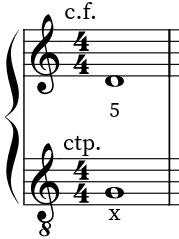
\includegraphics[height=1.3in]{Images/wrong_key.png}
        \caption{Ctp. not keeping the key tone set by the \cfdot}
        \label{fig:wrongkeytone}
    \end{figure}

    $G$ is used as a bass note to make a fifth instead of the $D$ note required to keep the key of the \cf \footnote{As it is, the work would be in $G$ Mixolydian instead of $D$ Dorian.}. This rule applies to all species.

    \item\label{rule:nounisson} \textit{The counterpoint and the \cf cannot play the same note at the same time except in the first and last measure.} \parencite[p.62]{GaPFr}

    It does not mean that the harmonic interval cannot be equal to zero because an octave can occur. But unison in the strict sense of the term cannot be used in this case. This rule applies to all species for all thesis\footnote{Thesis means the note on the downbeat.\label{fn:thesis}} notes.

    \item\label{rule:impconspref} \textit{Imperfect consonances\footnote{Imperfect consonances are thirds and sixths.} are preferred to perfect consonances.} \parencite[p.54]{GaPFr}

    Preferred means that all consonances are allowed but some cost, or "punishment", will be associated with the use of perfect consonances. This rule applies to all species for all thesis notes.

    \item\label{rule:low_penult} \textit{If the \cf is in the lower part, then the harmonic interval of the penultimate note must be a major sixth.} \parencite[p.54]{GaPFr}

    This rule seems a bit strange at first, but there is a rational explanation for this. Indeed, traditional \cf almost always end with a descending melody of one degree, for example, $E\to D$ or $F\to E$ (figure \ref{fig:descmelody}).
    \begin{figure}[h]
        \centering
        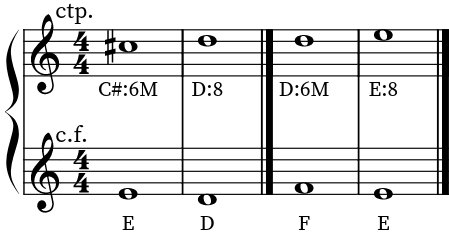
\includegraphics[height=\fh]{Images/penult_logic.png}
        \caption{\textit{Cantus firmus} ending with descending melodic intervals.}
        \label{fig:descmelody}
    \end{figure}

    From this example, the rule makes sense because the major sixths of $E$ and $F$ are $C\sharp$\footnote{$C\sharp$ is a leading-tone to $D$. Leading-tone is a note that resolves to the next note, one semitone higher (or lower). It begins to be used in the late Middle Ages \parencite{Leadingnote}.} and $D$ respectively. These notes are only one degree away from the tonic and lead perfectly by contrary motion to the tonics $E$ and $F$.
    However, this implies several things. First, if big leaps are to be avoided in general, the last consonance will necessarily be an octave or unison because, as explained above, the closest note is necessarily the tonic.
    
    Secondly, if a composer wants to use the tool to compose from a \cf that does not have the particularity of ending on a melody descending by one degree, then the solutions will not be very coherent on the penultimate measure. This point will be explained in more detail later. This rule applies to all species.
    
    \item\label{rule:up_penult} \textit{If the \cf is in the upper part, then the harmonic interval of the penultimate note must be a minor third.} \parencite[p.54]{GaPFr}

    This rule goes hand in hand with the previous one. Indeed, a minor third is an inverted major sixth\footnote{If the octave interval is defined by 12 semitones, then the minor third is 3 and the major sixth is 9. The same note is found because $(Cf-3)\ mod\ 12 = (Cf+9)\ mod\ 12$. In other words, any note is the minor third of its major sixth.}. With the previous example, the notes of the counterpoint used would be exactly the same but this time would be below the \cf (see figure \ref{fig:penultnotes1st}). This rule applies to all species.
    \begin{figure}[h]
        \centering
        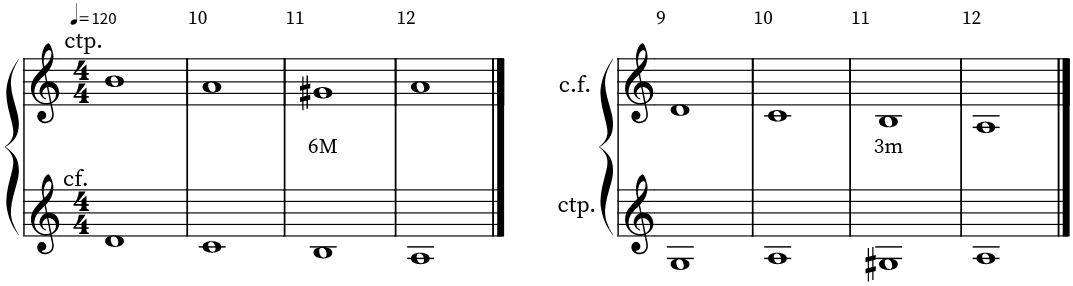
\includegraphics[height=\fh]{Images/penult_notes.png}
        \caption{Equivalence between \nth{6}M and \nth{3}m in penultimate measures, \species{1}.}
        \label{fig:penultnotes1st}
    \end{figure}
\end{enumerate}

\subsection{Melodic Rules of the First Species}
\begin{enumerate}[wide, label=\bfseries 1.M\arabic*]
    \item\label{rule:notritone} \textit{Tritone\footnote{If you want to hear what is a tritone, you can check the video \citetitle{TritoneYT} at \citeurl{TritoneYT} \parencite{TritoneYT}.} melodic intervals are forbidden.} \parencite[p.59]{GaPFr}

    The tritone, sometimes called the devil's interval by some \parencite[p.35]{GaPEng}, is a three-tone interval just below the perfect fifth \parencite{Tritone}. It brings a lot of dissonance that was often avoided in the melody. This is a common rule of classical music in the broad sense but it is more used in today's music, so it can be deactivated. This rule applies to all species.
    
    \item\label{rule:mlesixth} \textit{Melodic intervals cannot exceed a minor sixth interval.} \parencite[p.61]{GaPFr}
    \begin{quotation}
        "[The master addressing his pupil] You shouldn't be so impatient, though I am most glad about your care not to depart from the rules. But how should you avoid those small errors for which you have yet had no rules? [\dots] you used a skip of a major sixth, which is prohibited in strict counterpoint where everything should be as singable as possible."
        \textcite[p.37]{GaPEng}
    \end{quotation}

    As Fux explains, this rule applies especially to singers. As explained in rule \ref{rule:smallmelody}, it is not very melodious to make big leaps in the melody anyway. This rule applies to all species with some exceptions.
\end{enumerate}

\subsection{Motion Rules of the First Species}
\begin{enumerate}[wide, label=\bfseries 1.P\arabic*]
    \item\label{rule:nopconsbydm} \textit{Perfect consonances cannot be reached by direct motion.} \parencite[p.51, 57]{GaPFr}

    This rule is a good example of Fux overloading the explanations for perhaps a better understanding of the yesteryear audience.
    \begin{quote}
        "First rule: From one perfect consonance to another perfect consonance one must proceed in contrary or oblique motion.\\
        Second rule: From a perfect consonance to an imperfect consonance one may proceed in any of the three motions.\\
        Third rule: From an imperfect consonance to a perfect consonance one must proceed in contrary or oblique motion.\\
        Fourth rule: From one imperfect consonance to another imperfect consonance one may proceed in any of the three motions."
        \textcite[p.22]{GaPEng}
    \end{quote}

    As \textcite[p.23]{Esemplare} explains, these rules can be reduced to one such that the direct motion into perfect consonances is the only forbidden progression. Figure \ref{fig:perfectdirect} violates the rule. This rule applies to all species.
    \begin{figure}[h]
        \centering
        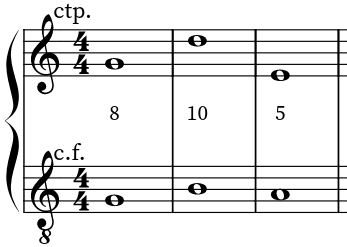
\includegraphics[height=\fh]{Images/direct_motion_pcons.png}
        \caption{Perfect consonance reached by direct motion.}
        \label{fig:perfectdirect}
    \end{figure}

    \item\label{rule:codmotions} \textit{Contrary motions are preferred to oblique motions which are preferred to direct motions.} \parencite[p.53]{GaPFr}
    
    According to Fux, this would avoid making mistakes. Since the purpose of counterpoint is to have different melodies, it is understandable that contrary motion is preferable as the melodies will naturally differ. He is nevertheless criticized for the use of oblique motions which are, by some authors, forbidden.

    \textcite{CpSachs} say that "The repetition of a note, causing oblique motion, is sometimes permitted only in the cantus, but may be used in either part (or even in both simultaneously, as a repeated note); it is not however the recommended ‘next step’."
    \textcite{ReglesJLFabre}\footnote{Jean-Louis Fabre has a long experience teaching and practicing music. He has taught piano, music writing, and analysis at the conservatory and more \parencite{BioJLFabre}.} explains that the treatises of Marcel Bitsch\parencite{Bitsch}, Marcel Dupré\parencite{Dupre}, or those of the 19th century, proscribe the repetition of a note.

    Since the preference of the motion is different according to the musical context, this parameter is manageable by the user. This rule applies to all species.
    
    \item\label{rule:battuta} \textit{At the start of any measure, an octave cannot be reached by the lower voice going up and the upper voice going down more than a third skip.} \parencite[p.61-62]{GaPFr}

    This rule may seem arbitrary because it is. The original rule forbids this \textit{battuta} octave\footnote{Literally translated from Italian to "beaten". It refers to the downbeat.} no matter how far the upper voice travels. Fux explains that "it is of little importance"\parencite[p.39]{GaPEng} because he has found no particular reason for this rule, which is respected by authoritative composers. However, he thinks that the octave reached by a leap in the same context should be avoided.
    \begin{figure}[h]
        \centering
        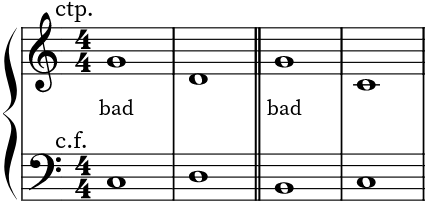
\includegraphics[height=\fh]{Images/battutas.png}
        \caption{Example of battuta octaves.}
        \label{fig:battuta}
    \end{figure}

    On the right of figure \ref{fig:battuta}, the octave is reached by a skip which is not good. While the example on the left is admitted by Fux. This rule applies to all species with some exceptions.
\end{enumerate}

\section{Formalization into Constraints}

\subsection{Harmonic Constraints of the First Species}

\paragraph{\ref{rule:allcons}} \textit{All harmonic intervals must be consonances.}

\begin{equation}
    \begin{gathered}
        \forall j \in [0, m)\quad 
        H[0, j] \in Cons
    \end{gathered}
\end{equation}
This can be expressed with the constraint {\small\texttt{(gil::g-member *sp* ALL\_CONS\_VAR h-intervals)}} (see original code for more details).

\paragraph{\ref{rule:firstpcons}, \ref{rule:lastpcons}} \textit{The first and last harmonic intervals must be a perfect consonances.}

\begin{equation}
    \begin{gathered}
        H[0, 0] \in Cons_{p}\\
        H[0, m-1] \in Cons_{p}
    \end{gathered}
\end{equation}

\paragraph{\ref{rule:keytone}} \textit{The key tone is tuned according to the first note of the \cfdot}

Rule \ref{rule:samekey} already handles the set of available additional notes. The only rule to add is that the first and last bass notes of the piece must have the same letter as the first note of the \cf (i.e. unison or octaves).

\begin{equation}
    \begin{gathered}
        \lnot IsCfB[0, 0] \implies H[0, 0] = 0\\
        \lnot IsCfB[0, m-1] \implies H[0, m-1] = 0
    \end{gathered}
\end{equation}

This is a good example of how implication works. {\small\texttt{RM\_IMP}} on code sample \ref{lst:tonictunedcst} means that the boolean to its left implies the relation again to its left.

\begin{lstlisting}[caption=Function that constrains the first and last harmonies to be unisons or octaves., label=lst:tonictunedcst, basicstyle=\ttfamily\scriptsize]
; @h-interval: the harmonic interval array
; @is-cf-bass-arr: boolean variables indicating if cf is at the bass
(defun add-tonic-tuned-cst (h-interval is-cf-bass-arr)
    (let (
        (bf-not (gil::add-bool-var *sp* 0 1)) ; s.f. !(first is-cf-bass-arr)
        (bl-not (gil::add-bool-var *sp* 0 1)) ; s.f. !(lastone is-cf-bass-arr)
    )
        ; bf-not = !(first is-cf-bass-arr)
        (gil::g-op *sp* (first is-cf-bass-arr) gil::BOT_EQV FALSE bf-not)
        ; bl-not = !(lastone is-cf-bass-arr)
        (gil::g-op *sp* (lastone is-cf-bass-arr) gil::BOT_EQV FALSE bl-not)
        ; bf-not => h-interval[0, 0] = 0
        (gil::g-rel-reify *sp* (first h-interval) gil::IRT_EQ 0 bf-not gil::RM_IMP)
        ; bl-not => h-interval[-1, -1] = 0
        (gil::g-rel-reify *sp* (lastone h-interval) gil::IRT_EQ 0 bl-not gil::RM_IMP)
)   )
\end{lstlisting}

Since the negation of IsCfBass is required and Gecode does not offer a $\lnot$ operation, it must be written in the form: $!p \equiv (p \iff \bot)$ where $p$ is any predicate (see lines 9 and 11).

\paragraph{\ref{rule:nounisson}} \textit{The counterpoint and the \cf cannot play the same note at the same time except in the first and last measure.}

\begin{equation}
    \begin{gathered}
        \forall j \in [1, m-1)\quad
        Cp[0, j] \neq Cf[j]
    \end{gathered}
\end{equation}

\paragraph{\ref{rule:impconspref}} \textit{Imperfect consonances are preferred to perfect consonances.}

Only the cost for perfect consonance is definable (\dft{low cost}) which leaves a null cost for the imperfect consonances.

\begin{equation}
    \begin{gathered}
        \forall j \in [0, m)\\
        Pcons_{costs}[j] = \begin{cases}
            cost_{Pcons} & \text{if } H[0, j] \in Cons_{p}\\
            0 & \text{otherwise}
        \end{cases}\\
        \text{moreover } \C = \C \cup \sum _{c \in Pcons_{costs}} c
    \end{gathered}
\end{equation}

\paragraph{\ref{rule:low_penult}, \ref{rule:up_penult}} \textit{The harmonic interval of the penultimate note must be a major sixth or a minor third depending on the \cf pitch.}

These two rules can be expressed with a single \textit{if-then-else} constraint like this: {\small\texttt{(gil::g-ite *sp* (penult *is-cf-bass-arr) NINE THREE (penult *h-intervals))}}.

\begin{equation}
    \begin{gathered}
        % \lnot IsCfB[0, m-2] \implies H[0, m-2] = 9
        \rho := \max (positions(m)) - 1\\
        H[\rho] = \begin{cases}
            9 & \text{if } IsCfB[\rho]\\
            3 & \text{otherwise}
        \end{cases}\\
        \text{where } \rho \text{ represents the penultimate index of any counterpoint.}
    \end{gathered}
\end{equation}

\subsection{Melodic Constraints of the First Species}

\paragraph{\ref{rule:notritone}} \textit{Tritone melodic intervals are forbidden.}

Instead of prohibiting this type of melodic interval, a cost is assigned (\dft{forbidden}) because it is a popular dissonant interval in today's music\footnote{Any major chord with a minor seventh has a tritone and this chord is the very basis of the blues \parencite{Seventhwiki}. It would be likely that users would arpeggiate on that with some melodic tritones.}. In addition, some less conventional \cf than those of Fux might require a tritone on the last motion because of the number of constraints on the penultimate measure. This cost is managed by the user in the same way as the other melodic interval costs as described in the general rule \ref{rule:smallmelody} at equation \ref{eq:mdeg_costs}.

\begin{equation}
    \begin{gathered}
        \forpm\\
        M[\rho] = 6 \implies Mdeg_{costs}[\rho] = cost_{tritoneMdeg}\\
    \end{gathered}
\end{equation}

\paragraph{\ref{rule:mlesixth}} \textit{Melodic intervals cannot exceed a minor sixth interval.}

\begin{equation}
    \begin{gathered}
        \forj\quad
        M[0, j] \leq 8
    \end{gathered}
\end{equation}

For simple rules that apply to the whole list, it is possible to add a single line constraint like this: {\small\texttt{(gil::g-rel *sp* m-intervals gil::IRT\_LQ 8)}.}

\subsection{Motion Constraints of the First Species}

\paragraph{\ref{rule:nopconsbydm}} \textit{Perfect consonances cannot be reached by direct motion.}

\begin{equation}
    \begin{gathered}
        \forj\quad
        H[0, j+1] \in Cons_{p} \implies P[0, j] \neq 2
    \end{gathered}
\end{equation}

This can be read as \emph{if a harmony belongs to the perfect consonances then the motion to reach it is not direct} ($2 \equiv direct$, see \textbf{P} in section \ref{sec:variables}).

\paragraph{\ref{rule:codmotions}} \textit{Contrary motions are preferred to oblique motions which are preferred to direct motions.}

\begin{multicols}{3}
    \begin{itemize}
        \item $cost_{con}$\\ \dft{no cost}
        \item $cost_{obl}$\\ \dft{low cost}
        \item $cost_{dir}$\\ \dft{medium cost}
    \end{itemize}
\end{multicols}

\begin{equation}
    \begin{gathered}
        \forj\\
        P_{costs}[j] = \begin{cases}
            cost_{con} & \text{if } P[0, j] = 0\\
            cost_{obl} & \text{if } P[0, j] = 1\\
            cost_{dir} & \text{if } P[0, j] = 2
        \end{cases}\\
        \text{moreover } \C = \C \cup \sum _{c \in P_{costs}} c
    \end{gathered}
\end{equation}

\paragraph{\ref{rule:battuta}} \textit{At the start of any measure, an octave cannot be reached by the lower voice going up and the upper voice going down more than a third skip.}

This rule can be represented by two sets of constraints. The first line of equation \ref{eq:battuta} represents the case where the counterpoint is on top while the second represents the case where the \cf is on top.

\begin{equation}
    \begin{gathered}
        i := \max (\B), \forj\\
        H[0, j+1] = 0 \land P[i, j] = 0 \land \begin{cases}
            M_{brut}[i, j] < -4 \land IsCfB[i, j] \iff \bot\\
            M_{cf}[i, j] < -4 \land \lnot IsCfB[i, j] \iff \bot
        \end{cases}\\
        \text{where } i \text{ stands for the last beat index in a measure.}
    \end{gathered}
    \label{eq:battuta}
\end{equation}